% Respaldo de la estructura utilizada para generar la figura 1.1; no se incluye en la compilación.
\begin{figuraNativa}[htbp]{Organigrama institucional y estructura operativa de audIT SpA}{1-organigrama}
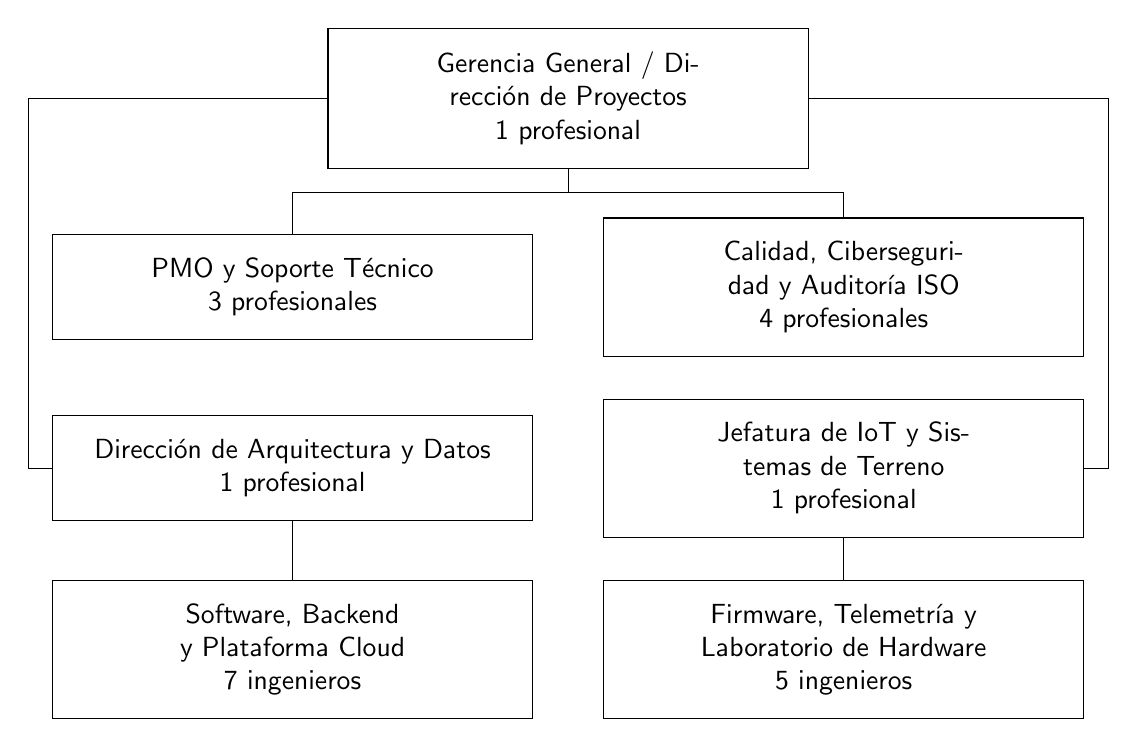
\begin{tikzpicture}[every node/.style={draw,text width=55mm,inner sep=3mm,align=center,font=\sffamily\fontsize{9.5bp}{12bp}\selectfont}]
\node (dg) at (0,0) {Gerencia General / Dirección de Proyectos\\1 profesional};
\node (pmo) at (-3.5,-2.4) {PMO y Soporte Técnico\\3 profesionales};
\node (qa) at (3.5,-2.4) {Calidad, Ciberseguridad y Auditoría ISO\\4 profesionales};
\node (arq) at (-3.5,-4.7) {Dirección de Arquitectura y Datos\\1 profesional};
\node (iot) at (3.5,-4.7) {Jefatura de IoT y Sistemas de Terreno\\1 profesional};
\node (sw) at (-3.5,-7.0) {Software, Backend y Plataforma Cloud\\7 ingenieros};
\node (hw) at (3.5,-7.0) {Firmware, Telemetría y Laboratorio de Hardware\\5 ingenieros};
\draw (dg.south) -- ++(0,-0.3) -| (pmo.north);
\draw (dg.south) -- ++(0,-0.3) -| (qa.north);
\draw (dg.west) -- ++(-3.8,0) |- (arq.west);
\draw (dg.east) -- ++(3.8,0) |- (iot.east);
\draw (arq.south) -- (sw.north);
\draw (iot.south) -- (hw.north);
\end{tikzpicture}
\par\smallskip Fuente: Estructura corporativa declarada por audIT. Dotación total: 22 personas.
\end{figuraNativa}
